\chapter{AI Component Design}
\label{ch:ai-component-design}

% 5.1
\section{Business Context and AI Integration}
\label{sec:business-context}

\begin{figure}[h]
    \centering
    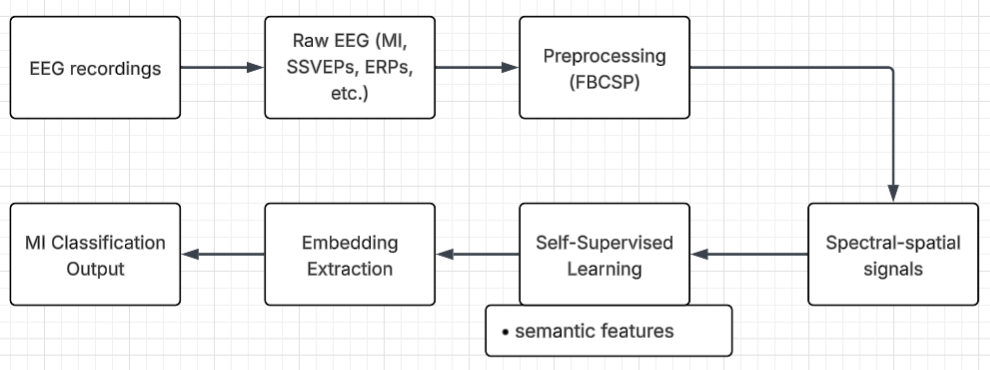
\includegraphics[width=0.95\textwidth]{figures/ssl-workflow}
    \caption{Self-supervised learning for semantic feature extraction from EEG signals.}
    \label{fig:ssl-workflow}
\end{figure}
\noindent

\vspace{1em}
\noindent\textbf{Diagram Explanation:}
The workflow begins with EEG recordings from multiple paradigms, including Motor Imagery (MI), SSVEPs, and ERPs. These raw signals undergo preprocessing using Filter Bank Common Spatial Pattern (FBCSP) to extract spectral-spatial features.
The resulting features are then passed into a self-supervised learning (SSL) module, which learns semantic embeddings from unlabeled EEG data.
These learned representations are later extracted and used for downstream MI classification, improving accuracy and generalization by leveraging knowledge from diverse EEG tasks.
\pagebreak

\vspace{1em}
\noindent\textbf{Why is AI suitable for this problem?}
\begin{itemize}
    \item EEG signals are complex, high-dimensional, and noisy.
    Rule-based or manually designed systems are not scalable or adaptable across paradigms.
\end{itemize}

\vspace{0.5em}
\noindent\textbf{Is the problem large, complex, or always changing?}
\begin{itemize}
    \item Yes.
    The system must generalize across multiple EEG types (MI, SSVEP, ERP) and accommodate unseen subjects and sessions.
    The input data structure and classification objectives can vary significantly.
\end{itemize}

\vspace{0.5em}
\noindent\textbf{Can we accept an answer that’s not 100\% perfect?}
\begin{itemize}
    \item Yes.
    In a research context, the goal is to improve MI classification performance over existing baselines.
    Absolute accuracy is not required — approximate, generalizable solutions are valuable.
\end{itemize}

%5.2
\section{Goal Hierarchy}
\label{sec:goal-hierarchy}

\noindent\textbf{Organizational Goal:} Advance EEG-based research and improve MI classification reliability with minimal annotation cost.

\vspace{0.5em}
\noindent\textbf{System Goal:} Enable EEG researchers to conduct multi-paradigm feature learning using a unified, self-supervised architecture.

\vspace{0.5em}
\noindent\textbf{User Goal:} Simplify the research process by automating preprocessing, training, evaluation, and comparison through an integrated system.

\vspace{0.5em}
\noindent\textbf{AI Model Goal:} Learn general-purpose EEG embeddings using contrastive SSL and boost MI classification accuracy using transferred representations.

\vspace{1em}
\noindent\textbf{Success Metrics:}
\begin{itemize}
    \item Accuracy, F1-score, Precision, Recall.
    \item Robust cross-subject generalization.
    \item Automation of model training with minimal user input.
\end{itemize}

%5.3
\section{Task Requirements Analysis Using AI Canvas}
\label{sec:ai-canvas}

\subsection{AI Task Requirements}
\label{subsec:ai-task-requirements}
\begin{itemize}[leftmargin=3.5em]
    \item \textbf{Requirements (REQ):} Learn semantic EEG features across MI, SSVEP, and ERP signals using unlabeled data.
    \item \textbf{Specifications (SPEC):} Investigate how SSL-based representations improve MI classification accuracy and generalization.
    \item \textbf{Environment (ENV):} Evaluated using EEG datasets like BCIC2a and OpenBMI under varying conditions (e.g., noise, subject variation).
\end{itemize}

\subsection{AI Canvas Summary}
\label{subsec:ai-canvas-summary}
\begin{itemize}[leftmargin=3.5em]
    \item \textbf{Input:} EEG signal segments from multiple paradigms (preprocessed).
    \item \textbf{Output:} Semantic embeddings and MI class predictions.
    \item \textbf{Success Criteria:} $>$80\% accuracy on unseen subjects; generalization across tasks and datasets.
\end{itemize}

\subsection{Innovation}
\label{subsec:innovation}
\begin{itemize}[leftmargin=3.5em]
    \item A unified self-supervised learning pipeline capable of integrating diverse EEG paradigms (MI, SSVEPs, ERPs) into a common representation space.
\end{itemize}

\pagebreak
%5.4
\section{User Experience Design with AI}
\label{sec:ux-ai}

The proposed system is designed to offer a seamless and fully automated user experience, allowing researchers to interact with complex AI pipelines without needing deep programming knowledge.
The goal is to minimize manual configuration while preserving flexibility for experimentation.

\vspace{1em}
\noindent\textbf{Interface Overview:}
The user interface is divided into four main functional tabs — Train, Predict, Evaluate, and Compare — each offering a focused and intuitive workflow.

\begin{itemize}[leftmargin=3.5em]
    \item \textbf{Train Tab:} Allows users to select EEG datasets, configure SSL models, set hyperparameters (e.g., learning rate, epochs), and initiate training.
    A real-time training log displays progress and final performance.
    \item \textbf{Predict Tab:} Users can upload EEG samples and receive predictions including predicted class and confidence scores.
    \item \textbf{Evaluate Tab:} After uploading a trained model, users can view evaluation metrics such as accuracy, precision, recall, and F1-score, as well as a training loss/accuracy curve.
    \item \textbf{Compare Tab:} Enables side-by-side model comparison (e.g., SSL vs supervised) with metric summaries and bar chart visualizations.
\end{itemize}

\vspace{1em}
\noindent\textbf{System Behavior:}
Upon user interaction, the backend automatically executes preprocessing, training, evaluation, and result generation.
Logs, graphs, and final metrics are dynamically updated and available for export.

\vspace{1em}
\noindent\textbf{Feedback Loop:}
The system encourages iterative research workflows.
Users can adjust hyperparameters, change datasets, and refine model settings based on prior experimental outcomes.

\noindent\textbf{Interface Screenshots:}

\begin{figure}[H]
    \centering
    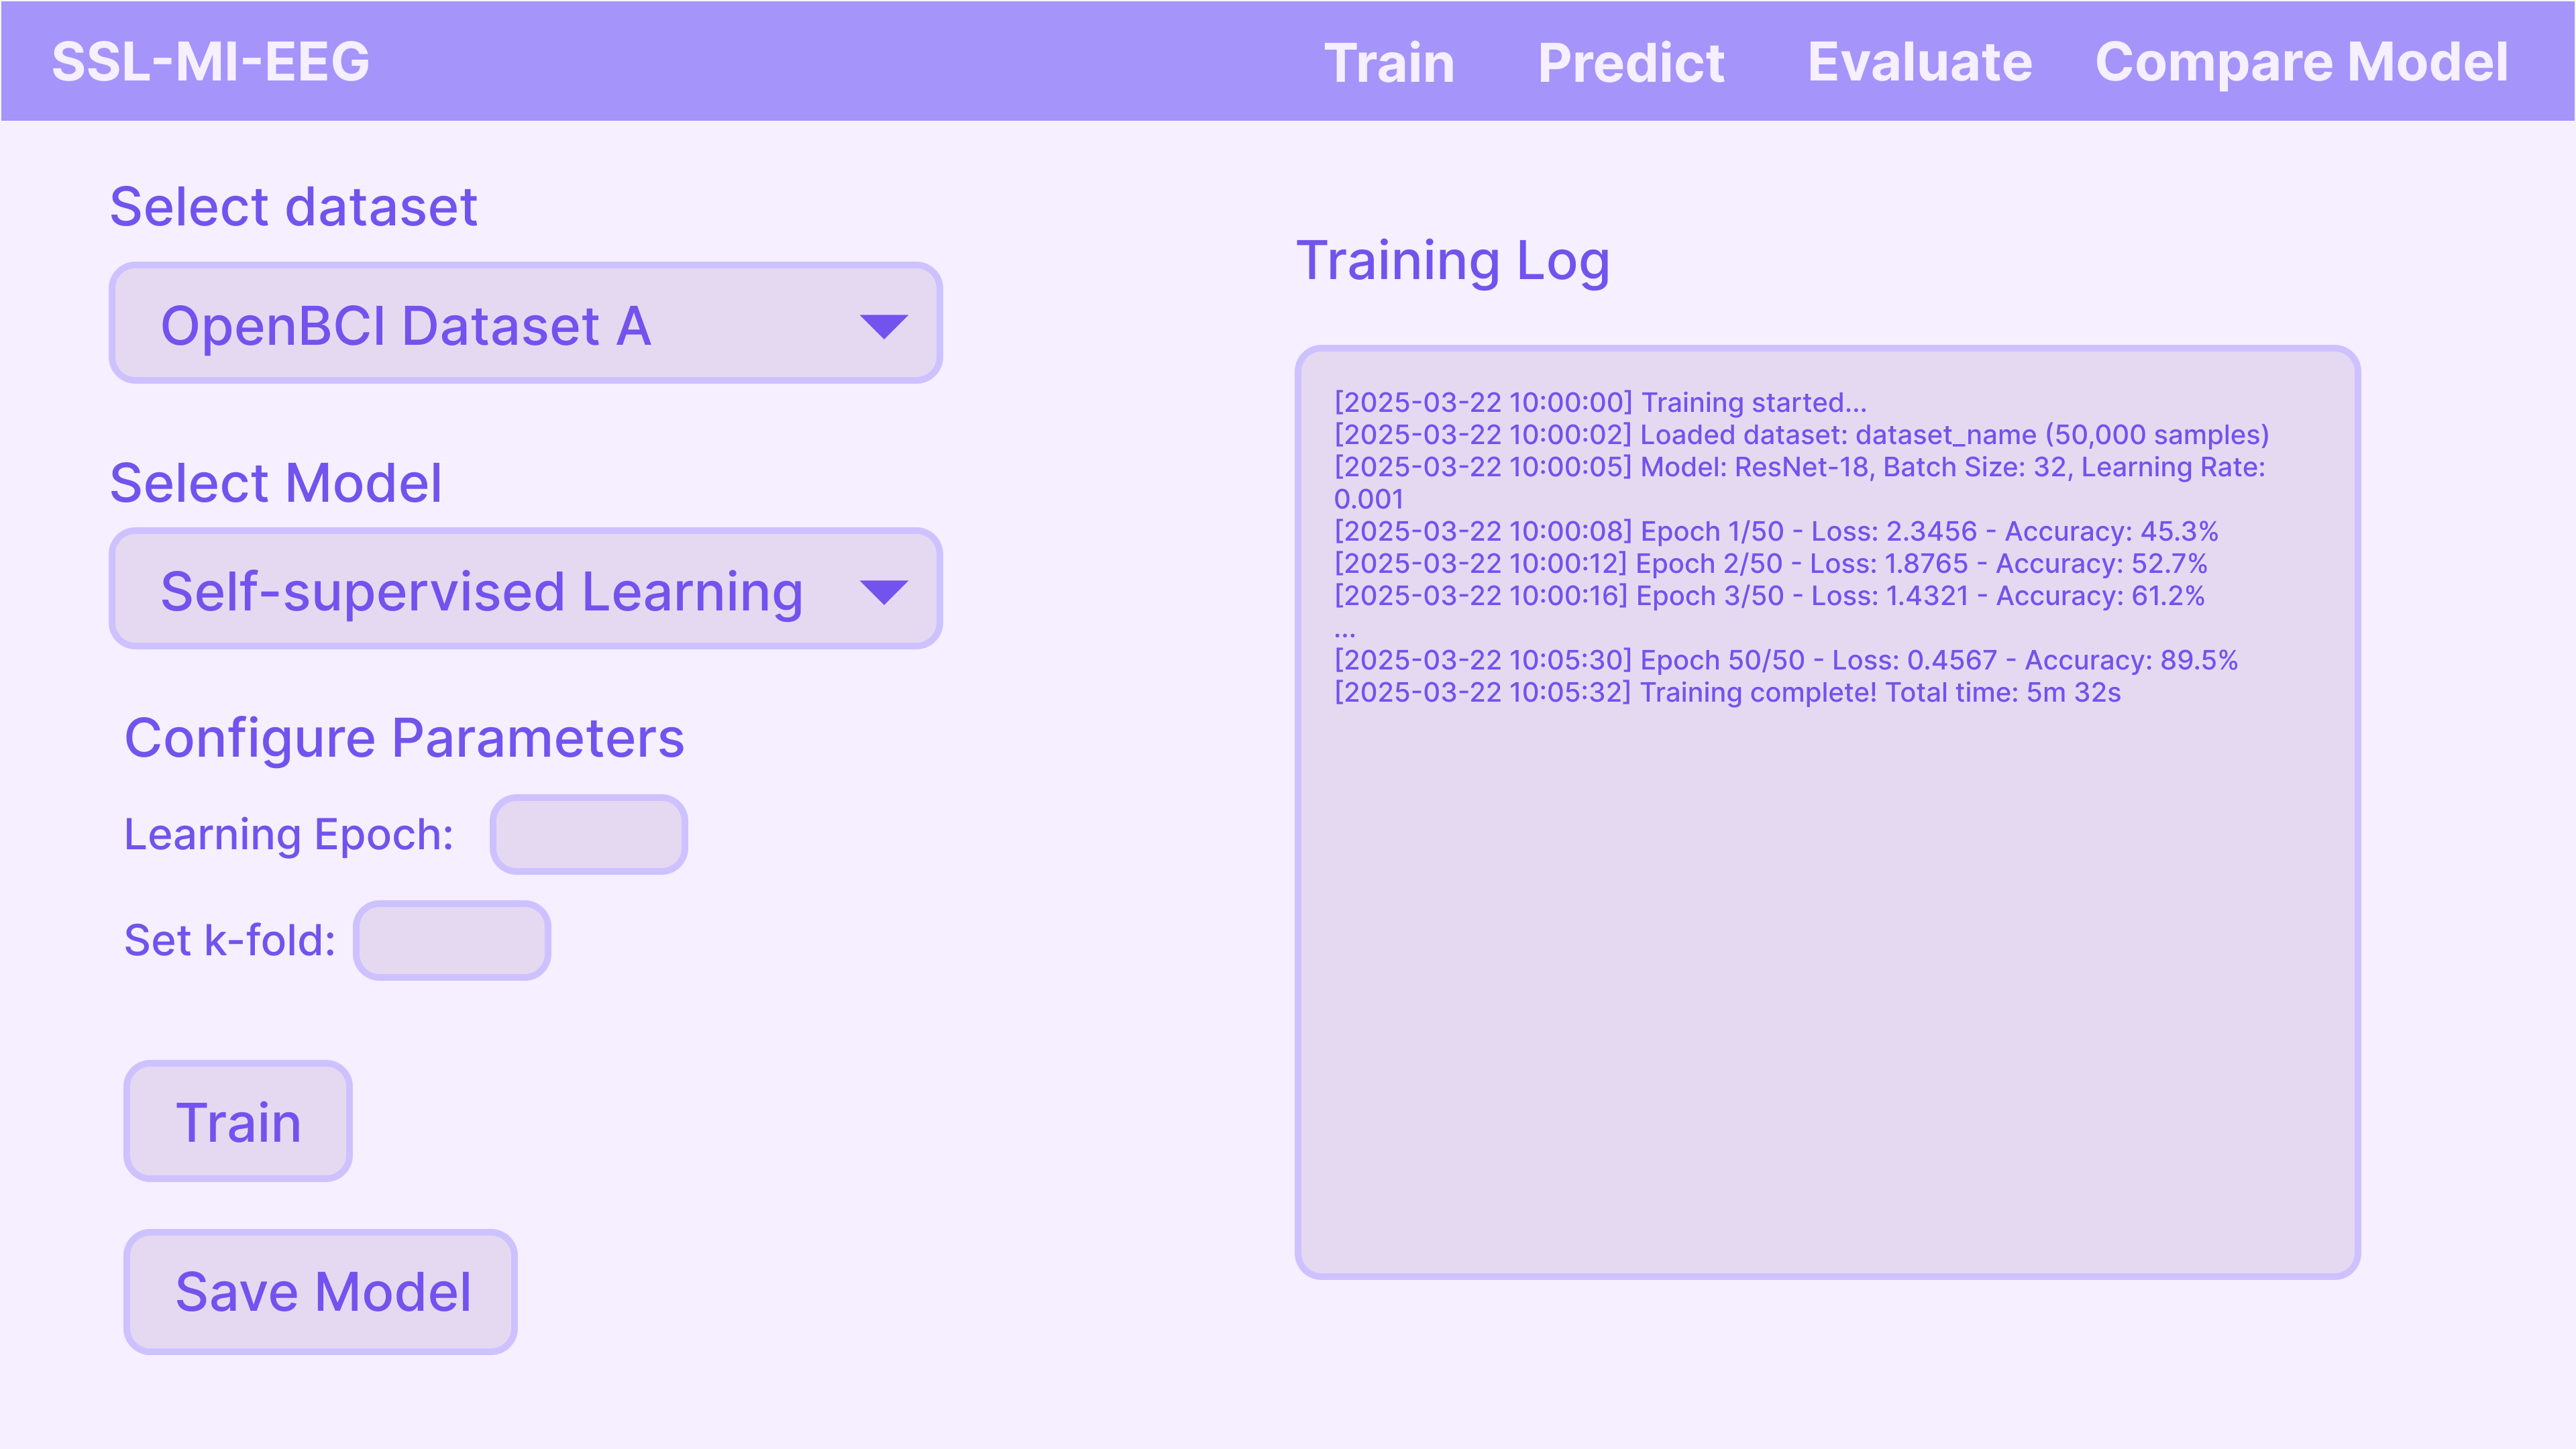
\includegraphics[width=0.9\textwidth]{figures/ui/train_model}
    \caption{Training Interface – Dataset selection, SSL configuration, and training log}
    \label{fig:ui_train_model}
\end{figure}

\begin{figure}[H]
    \centering
    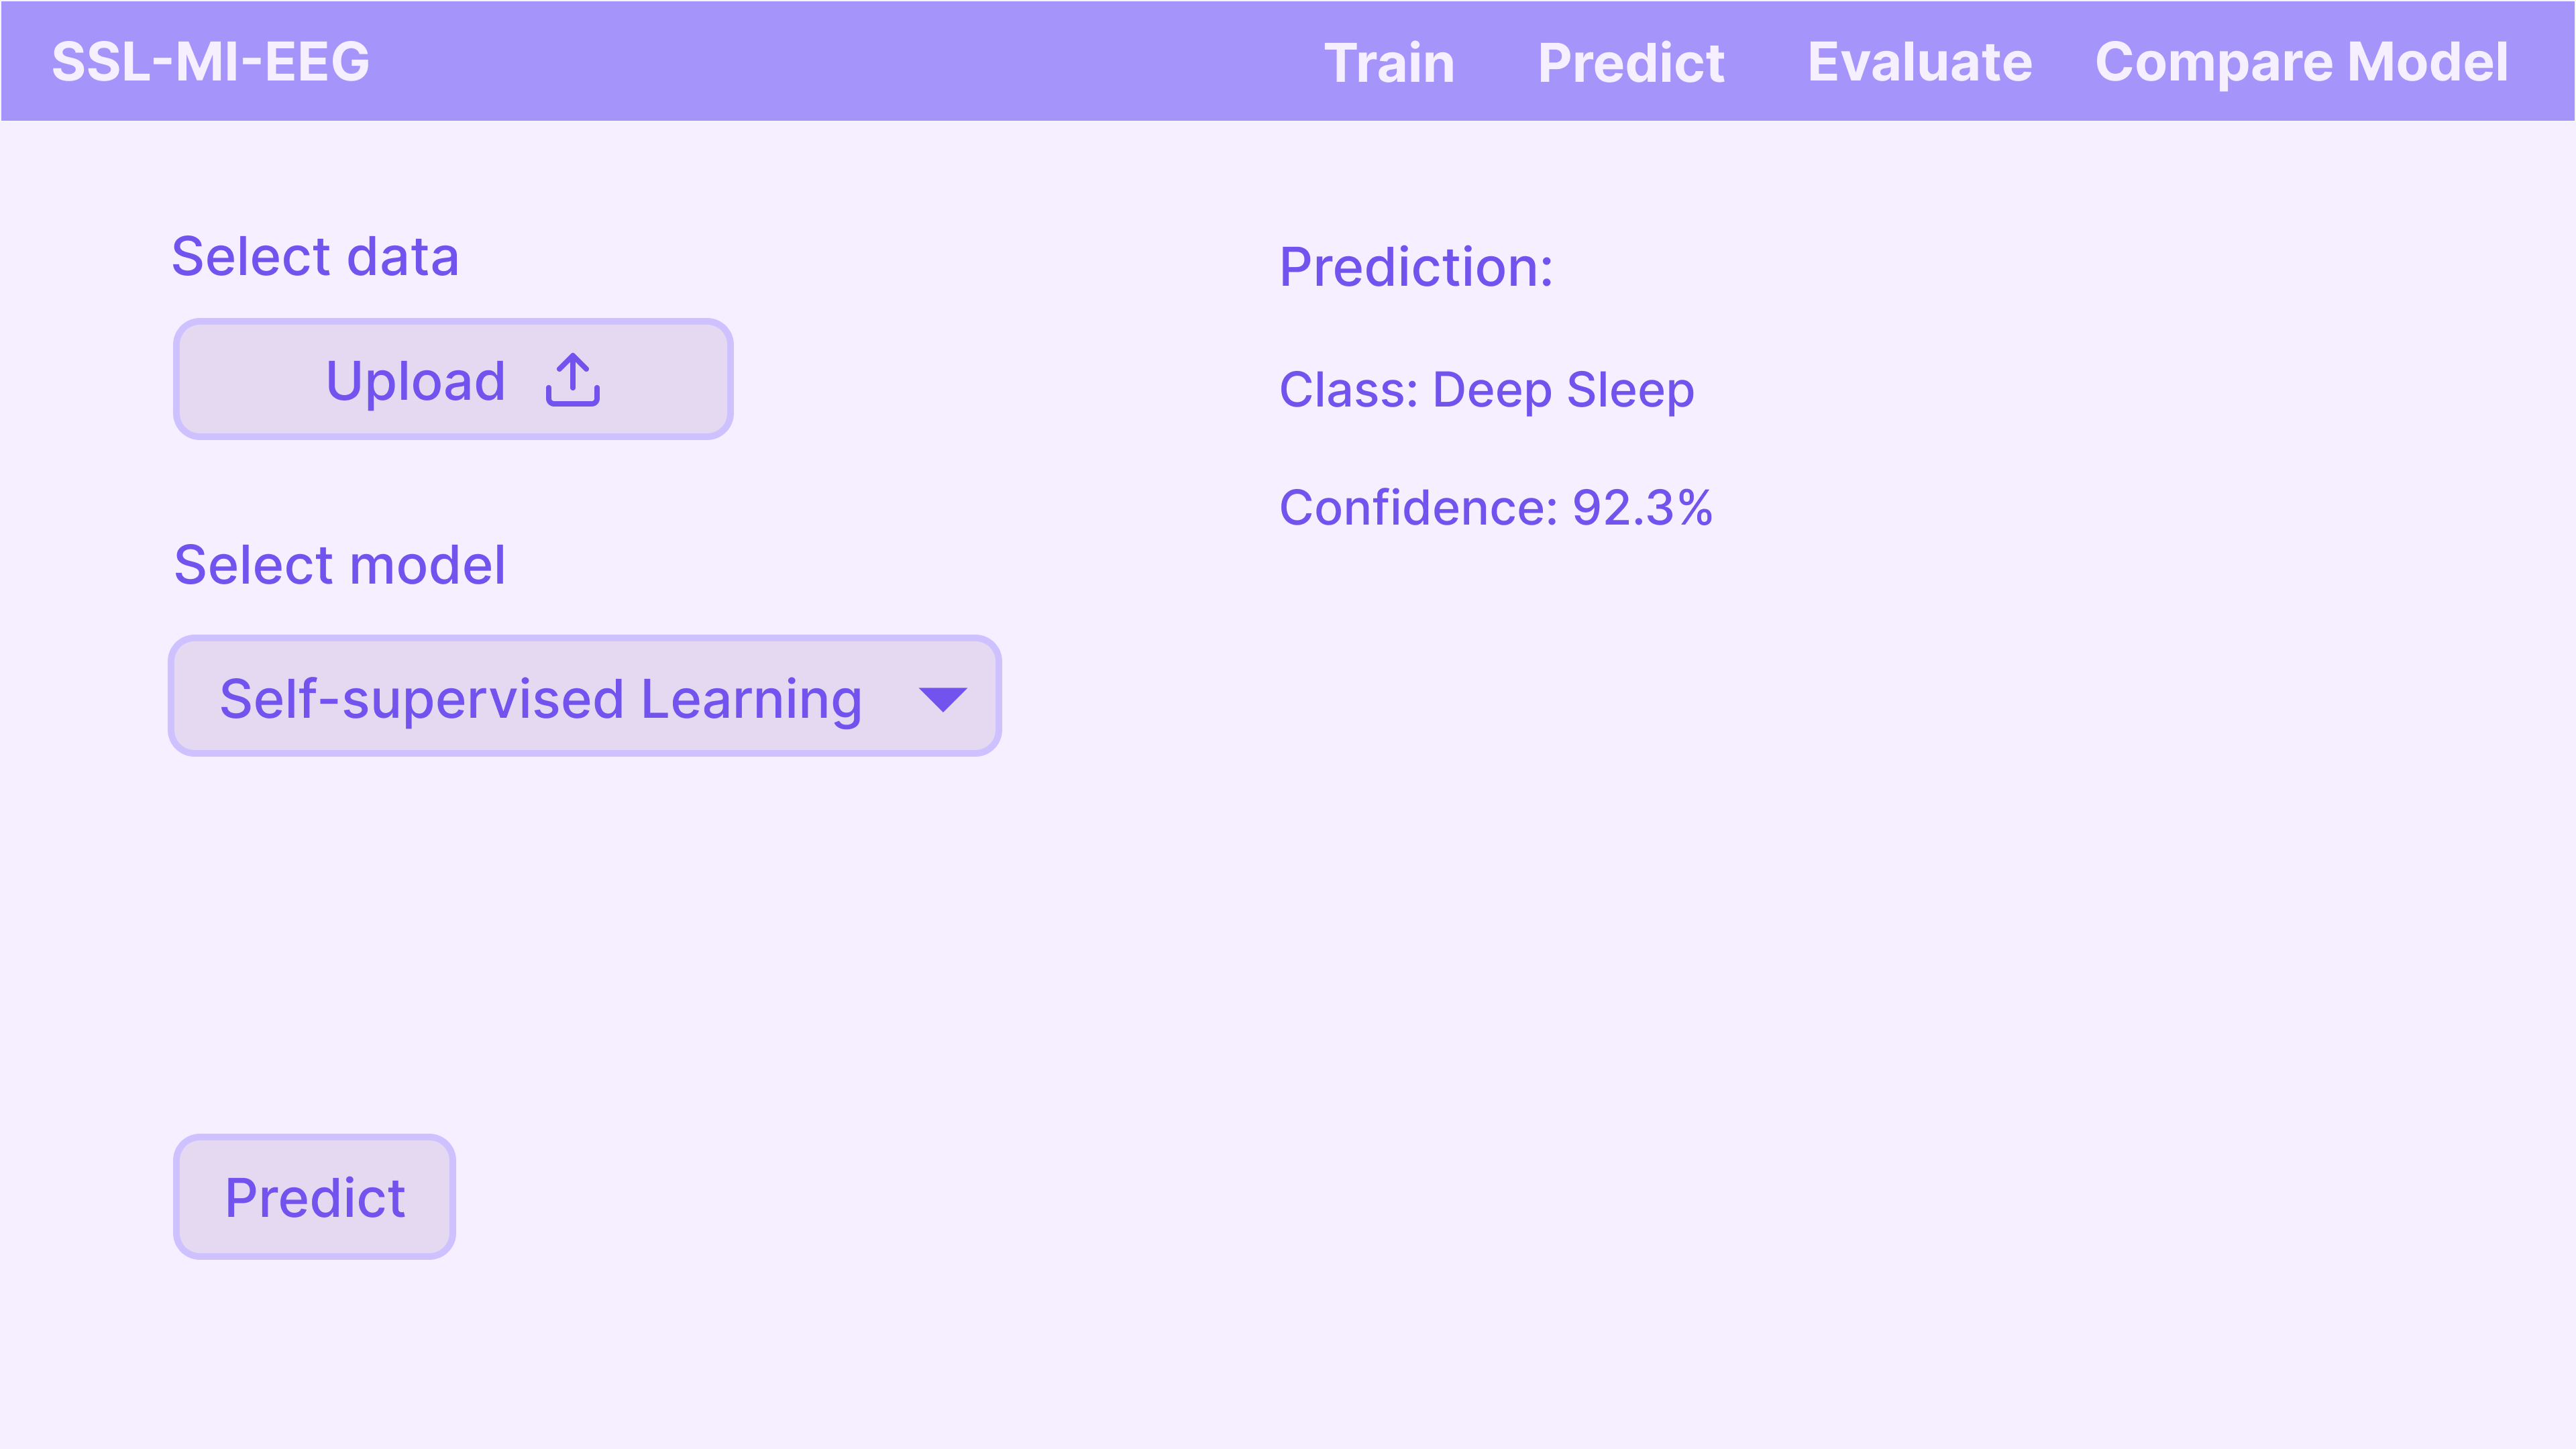
\includegraphics[width=0.9\textwidth]{figures/ui/predict_model}
    \caption{Prediction Interface – Uploading input data and viewing output class with confidence}
    \label{fig:ui_predict_model}
\end{figure}

\begin{figure}[H]
    \centering
    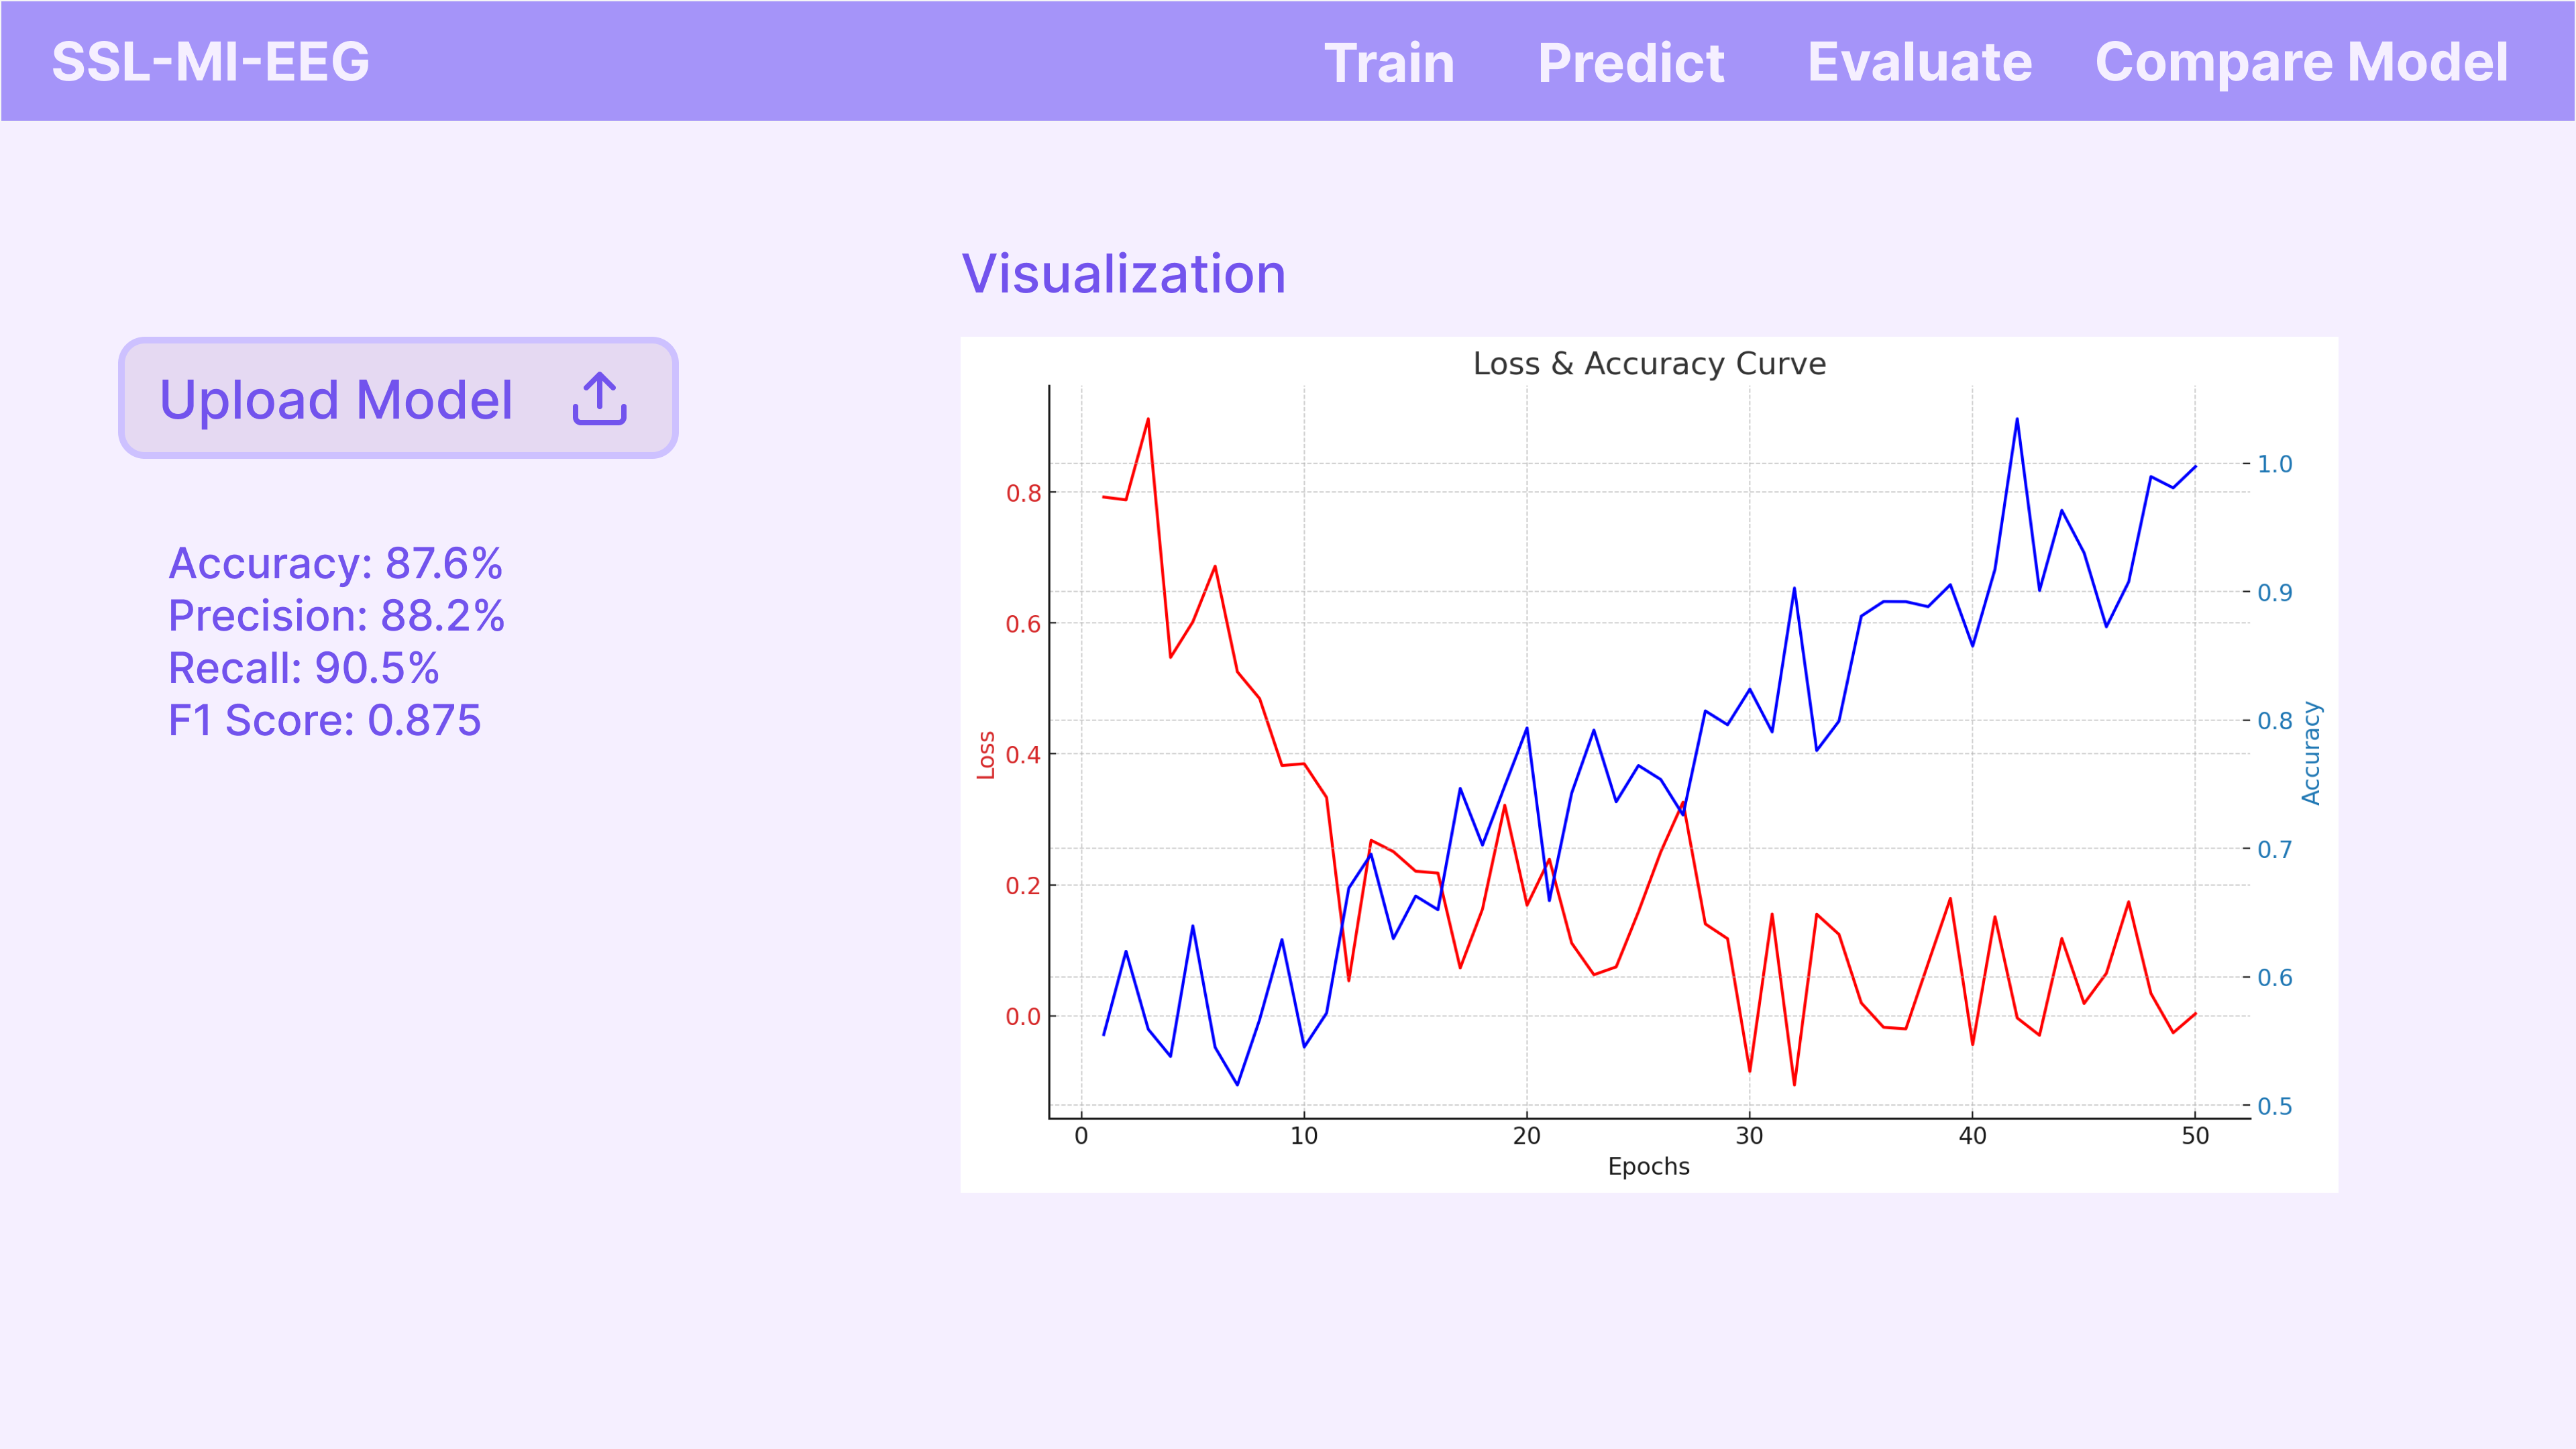
\includegraphics[width=0.9\textwidth]{figures/ui/evaluate_model}
    \caption{Evaluation Interface – Upload trained model and view performance metrics and curve}
    \label{fig:ui_evaluate_model}
\end{figure}

\begin{figure}[H]
    \centering
    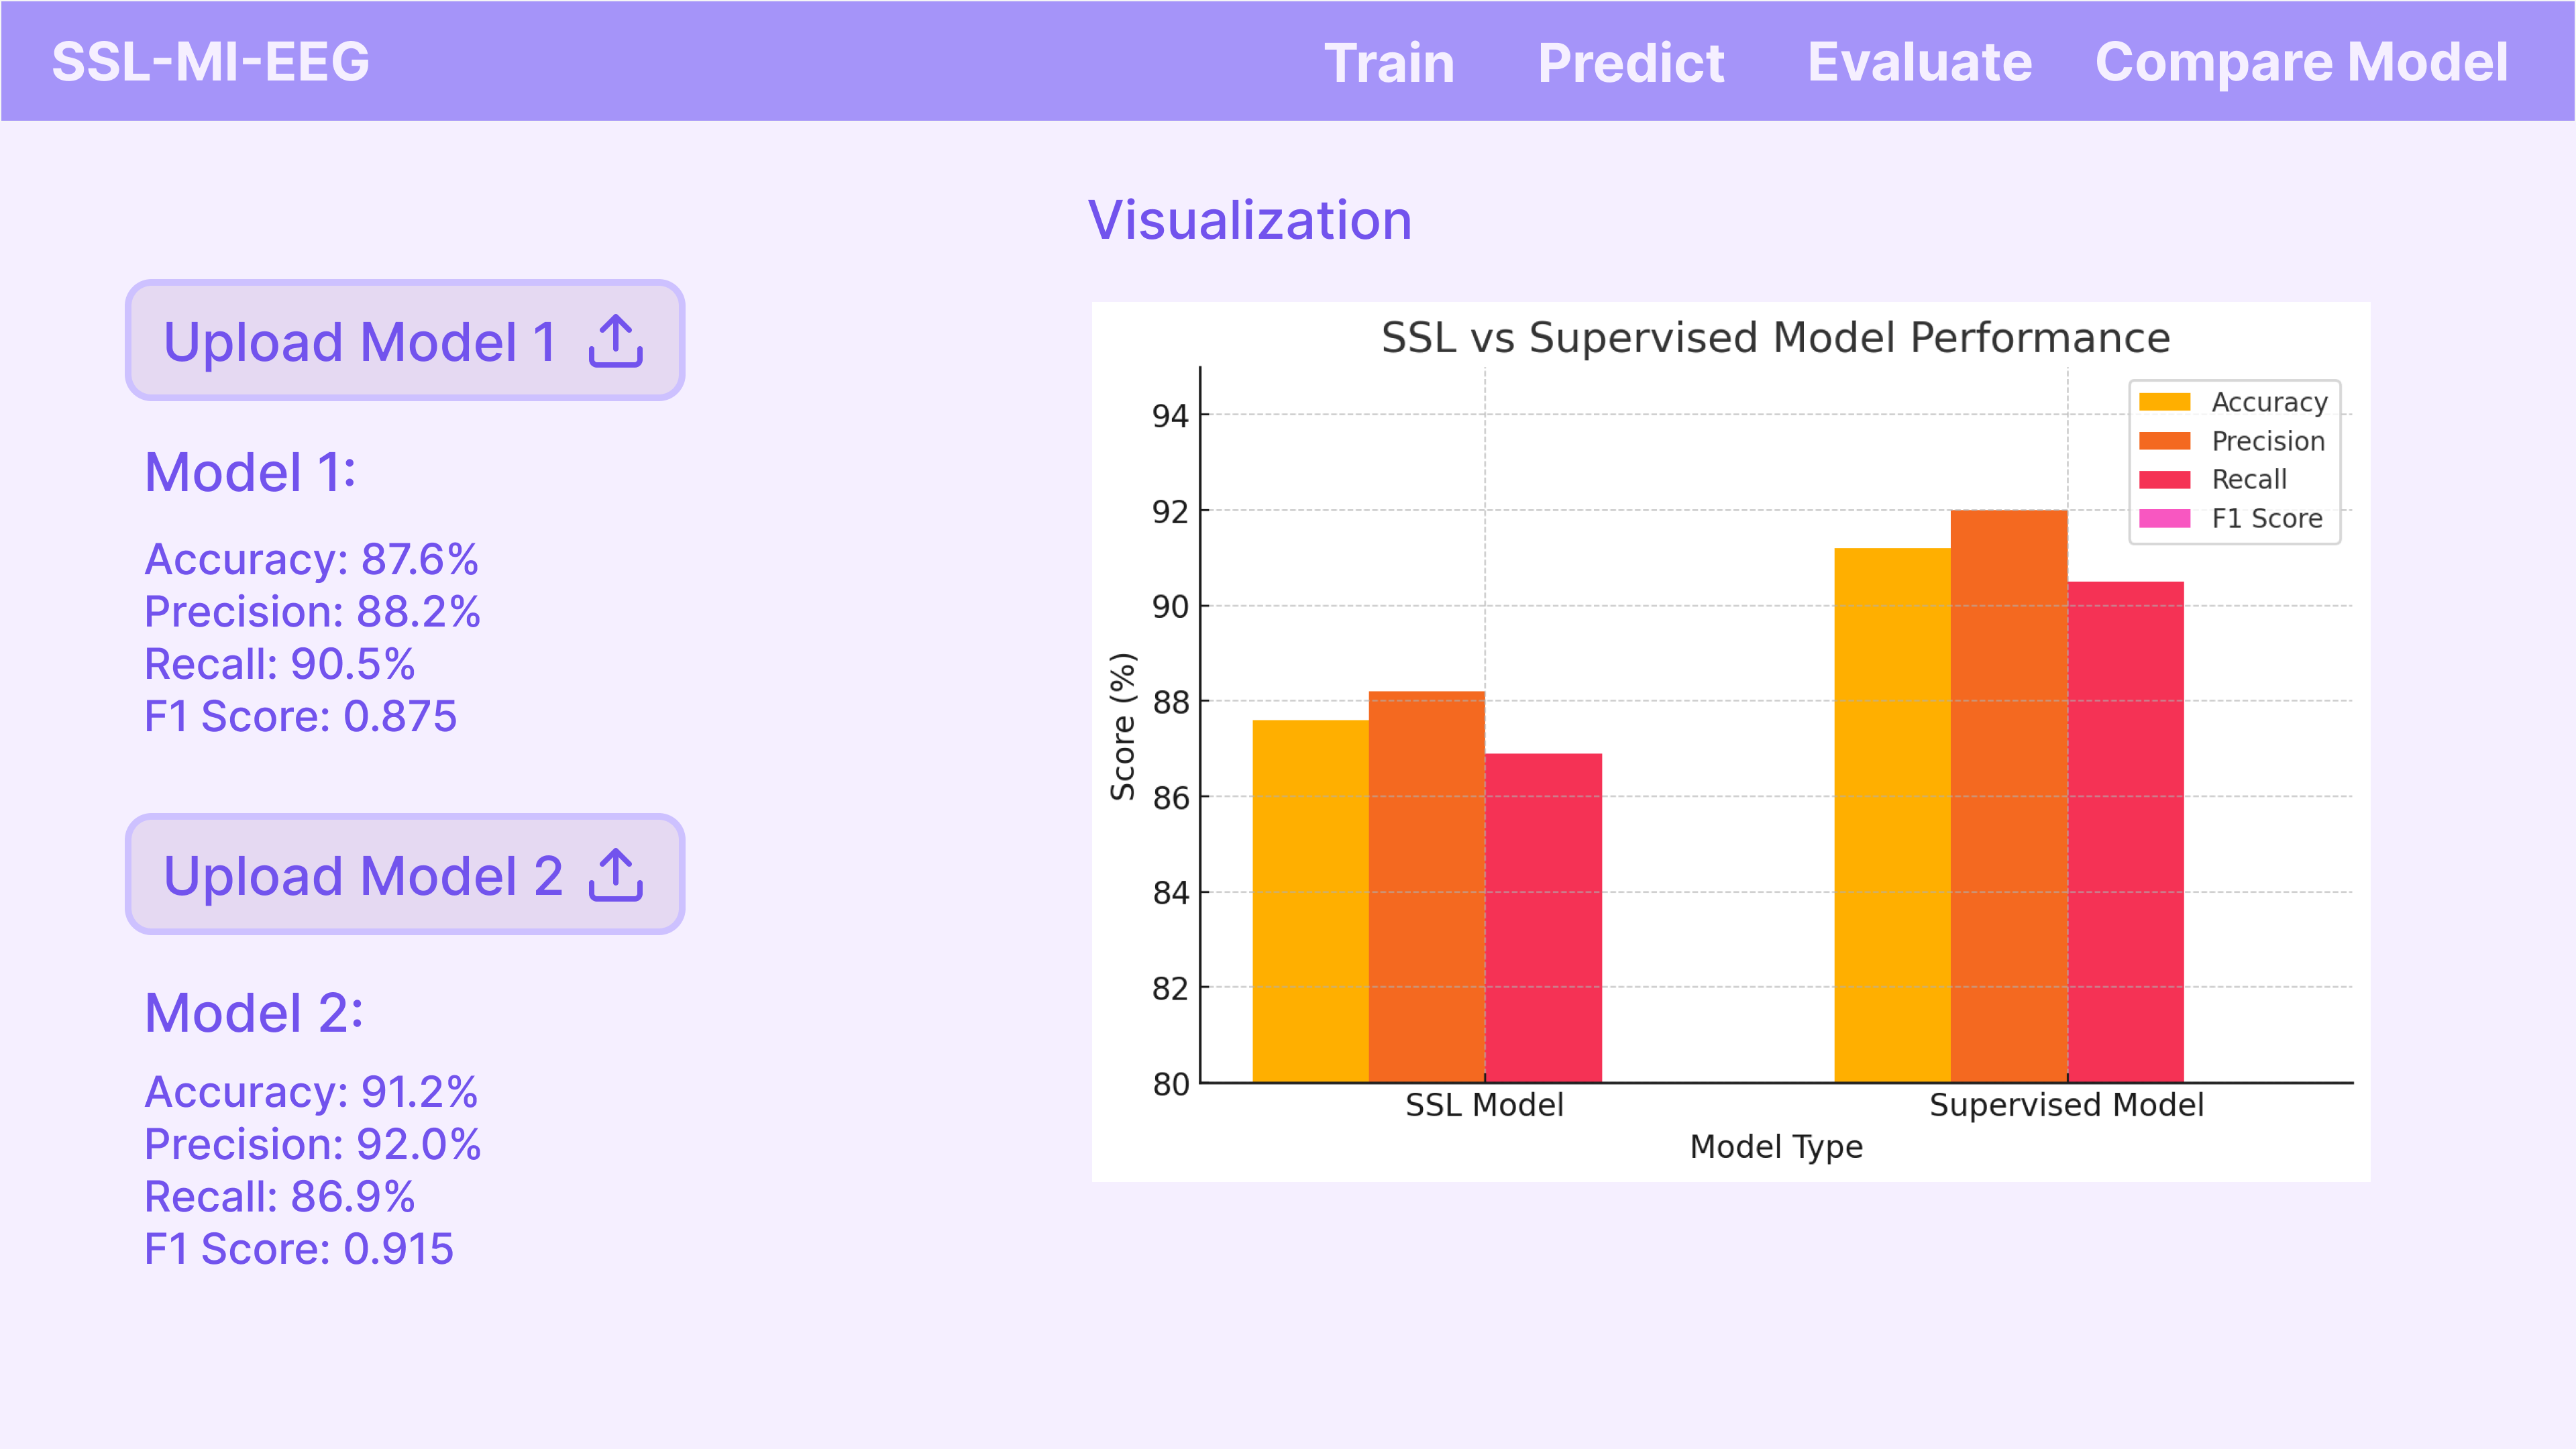
\includegraphics[width=0.9\textwidth]{figures/ui/compare_model}
    \caption{Comparison Interface – Visual comparison between SSL and Supervised models}
    \label{fig:ui_compare_mode}
\end{figure}

\FloatBarrier


%5.5
\section{Deployment Strategy}
\label{sec:deployment-strategy}

\subsection{Deployment Plan}
\label{subsec:deployment-plan}
The AI component in this project is developed for research purposes and is deployed in controlled environments: on local machines and on Google Colab.
This setup allows for flexible experimentation, reproducibility, and access to GPU acceleration when needed.

The core model used in our system is based on \textbf{MixNet-BCI}, an open-source EEG classification framework developed by VISTEC. This model is integrated into our workflow for signal preprocessing, feature extraction, and classification of motor imagery tasks.

System interaction is supported through a local \textbf{FastAPI} server, which simulates integration with other software components.
RESTful endpoints are used to send EEG data and receive classification results, mimicking real-world application scenarios in a lightweight and modular fashion.

The following tools and frameworks are used in our deployment:
\begin{itemize}
    \item \textbf{MixNet-BCI (VISTEC)} — for model architecture and EEG classification.
    \item \textbf{FastAPI} — for exposing the AI model via REST API endpoints.
    \item \textbf{Google Colab} — for cloud-based training and evaluation using GPU resources.
    \item \textbf{TensorFlow, TensorFlow Addons} — for low-level deep learning operations.
    \item \textbf{scikit-learn, pandas, h5py} — for data preprocessing and analysis.
    \item \textbf{mne, moabb} — for EEG signal handling and benchmarking against standard datasets.
\end{itemize}

The system is designed to be \textbf{easy to use}, especially for researchers.
With ready-to-run Colab notebooks, pre-defined functions, and simple API access, users can quickly run experiments, modify parameters, and analyze results without complex setup or infrastructure.

\subsection{Proof of Concept}
\label{subsec:proof-of-concept}
To validate the AI component, we integrated MixNet-BCI into our processing pipeline and tested it using the BCI Competition IV-2a dataset.
We experimented with two configurations:
\begin{itemize}
    \item \textbf{Subject-Dependent Setting:} Model is trained and tested on individual subjects.
    \item \textbf{Subject-Independent Setting:} Model is trained on a group of subjects and tested on unseen individuals.
\end{itemize}

This proof of concept demonstrates that MixNet-BCI, combined with our deployment strategy, effectively supports EEG-based motor imagery classification in a modular and research-ready environment.
Outputs are visualized within Jupyter/Colab notebooks, and inference can be accessed through the FastAPI interface for integration testing.


%5.6
\section{Reflection and Future Development}
\label{sec:reflection}


\subsection*{Lessons Learned}
\begin{itemize}[leftmargin=3.5em]
    \item SSL can extract high-quality embeddings from unlabeled EEG data that generalize to MI classification tasks.
    \item Multi-paradigm training (e.g., SSVEP + ERP) provides richer features than MI alone.
\end{itemize}


\subsection*{Challenges}
\begin{itemize}[leftmargin=3.5em]
    \item Temporal alignment and signal variability across EEG paradigms.
    \item Visualizing and interpreting high-dimensional learned representations.
\end{itemize}

\subsection*{Future Work}
\begin{itemize}[leftmargin=3.5em]
    \item Introduce transformer-based models for long-range EEG dependencies.
    \item Deploy a live MI classification demo with real-time prediction.
\end{itemize}
